\documentclass{beamer}
\usetheme{Boadilla}
\usepackage[utf8]{inputenc}
\usepackage{amsmath}
\usepackage{amsfonts}
\usepackage{amssymb}
\usepackage{cite}
\usepackage{graphicx}
\author{Ryan Honea}
\title[SVM For Classification]{Support Vector Machines for Classification \\ \large Applications with Random Point Clouds and Image Sets}
%\setbeamercovered{transparent} 
%\setbeamertemplate{navigation symbols}{} 
%\logo{} 
\institute{Austin Peay State University} 
\date{December 8th, 2017}
%\subject{} 

\AtBeginSection[]{
  \begin{frame}
  \vfill
  \centering
  \begin{beamercolorbox}[sep=8pt,center,shadow=true,rounded=true]{title}
    \usebeamerfont{title}\insertsectionhead\par%
  \end{beamercolorbox}
  \vfill
  \end{frame}
}
\begin{document}

\begin{frame}
\titlepage
\end{frame}

\begin{frame}[allowframebreaks]
\tableofcontents
\end{frame}

\section{Introduction}

\subsection{Definition of a Classification Problem}
\begin{frame}{The Classification Problem}
Defining the Classification Problem:

\begin{itemize}
\item Consider a set of elements $A$ that contains two subsets of elements defined as $A^-$ and $A^+$.
\item Let $x_1, ..., x_n \in A^+$ and let $y_1, ..., y_n \in A^-$
\item Now let $z \in A$, but it is unknown whether or not $z \in A^+$ or $z \in A^-$.
\item The objective of a classification problem is to define some rule that could determine the subset in which $z$ lies.
\item This problem can be generalized to have a set of elements $A$ with $n$ subsets and determining which subset $A^n$ that $z$ is an element of.
\item Typically, an $n$-subset decision problem requires $n-1$ decision boundaries.
\end{itemize}
\end{frame}

\subsection{Bayes Decision Rule}
\begin{frame}{Decision Rules and Boundaries}
We can define a general decision rule as such
$$z \in \begin{cases}A^-,& \text{if }P(A^-|z) > P(A^+|z)\\
A^+,& \text{otherwise}\end{cases}$$
but perhaps a more specific version utilizing Baye's Formula
$$z \in \begin{cases}
A^-, & \text{if } P(z|A^-)P(A^-) > P(z|A^+)P(A^+)\\
A^+, & \text{ otherwise}
\end{cases}$$
These decision rules are a generalization of Bayes' Decision Rules. In it's most simple form that assumes independence and randomness of elements, an algorithm called Naive Bayes determines what subset $z$ belongs to.
\end{frame}

\subsection{Support Vector Machines}
\begin{frame}{Define the Support Vector Machine}
\begin{itemize}
\item Again, consider a set of elements $A$ with subsets $A^-$ and $A^+$ with elements $\vec{x_-} \in A^-$ and $\vec{x_+} \in A^+$.
\item The objective in using Support Vector Machines is to create a hyperplane $\omega$ that intersects the set of elements $A$ in such a way that the distance $d$ from the closest point of $A^-$ and $A^+$ to $\omega$ is maximized.\nocite{Cortes1995}\nocite{mit_2014}
\item That is, we seek to find $\omega$ that maximizes $d$
\item We then define a new term $$y_i = \begin{cases}+1, &\text{if } x_i \in A^+\\ -1, & \text{ o/w}\end{cases}$$
\end{itemize}
\end{frame}

\begin{frame}{Maximizing Distance}
\begin{itemize}
\item This creates the following decision rule, where $\vec{v}$ is a vector that is perpendicular to $\omega$
$$\text{If } v_i * x_i \text{ is beyond the decision boundary, } x_i \in A^+$$
\item This idea defines two constraints
$$\vec{v}\cdot\vec{x_+} + b \geq +1$$
$$\vec{v}\cdot\vec{x_-} + b \leq -1$$
\item This constraint is simplified by $y_i$ to be
$$y_i(v_i \cdot x_i + b) \geq 1$$
\end{itemize}
\end{frame}

\begin{frame}{Quadratic Programming}
Because $\vec{v}$ is unknown, we seek to find $\vec{v}$ such that $d$ is maximized. For sake of time, this becomes a quadratic programming problem that seeks to solve
\begin{equation*}
v(\alpha) = \sum_i^n \alpha_i - \sum_i^n\sum_j^n \alpha_i \alpha_j y_i y_j \vec{x}_i^T \vec{x}_j
\end{equation*}
\begin{equation*}
\sum_i^n \alpha_iy_i = 0, \quad \quad \alpha_i \geq 0
\end{equation*}
There are a number of ways to maximize $\vec{v}$ through quadratic programming, and those are all a key part of the algorithm.
\end{frame}

\subsection{The Machine Learning Method}
\begin{frame}{Training, Testing Datasets}
Steps to Machine Learning
\begin{enumerate}
\item Define a training subset and testing subset of data
\item Define decision boundary based on training subset
\item Predict on the testing subset and calculate accuracy/error
\item If low accuracy, attempt other methods and repeat steps 1-3
\end{enumerate}
\end{frame}

\section{The Linear Case}
\subsection{Example Point Cloud}
\begin{frame}{Solving the Linear Case}
Objectives
\begin{itemize}
\item In the linear case, we try to draw a straight line through a series of points to define the hyperplane
\item We use the algorithm to define the plane
\item Example points:
\begin{center}
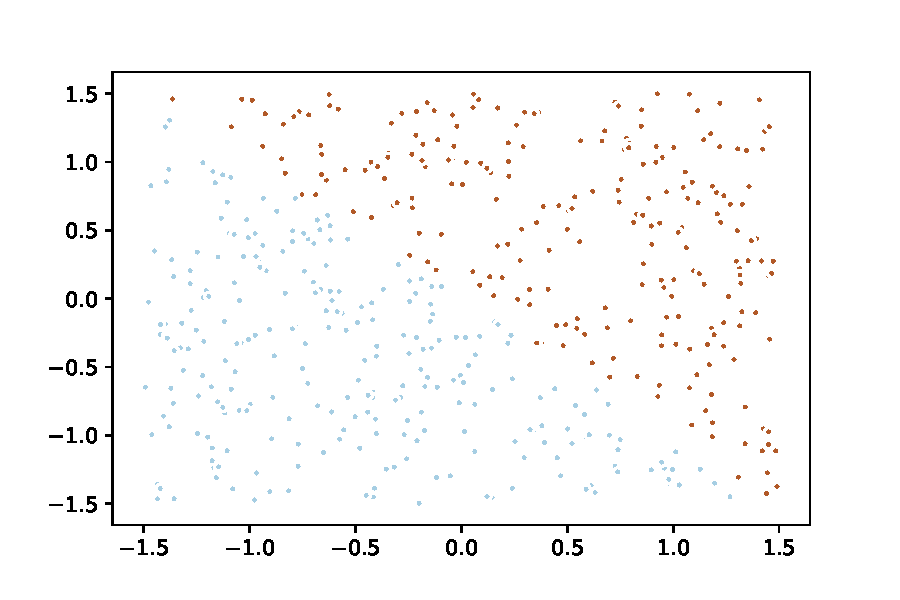
\includegraphics[scale=.6]{examples.pdf}
\end{center}
\end{itemize}
\end{frame}

\subsection{Results}
\begin{frame}{Results}
\begin{itemize}
\item In this case the testing subset is 50\% of the data and the training subset is the other 50\% of the data
\item Errors in testing are represented by red edges
\begin{center}
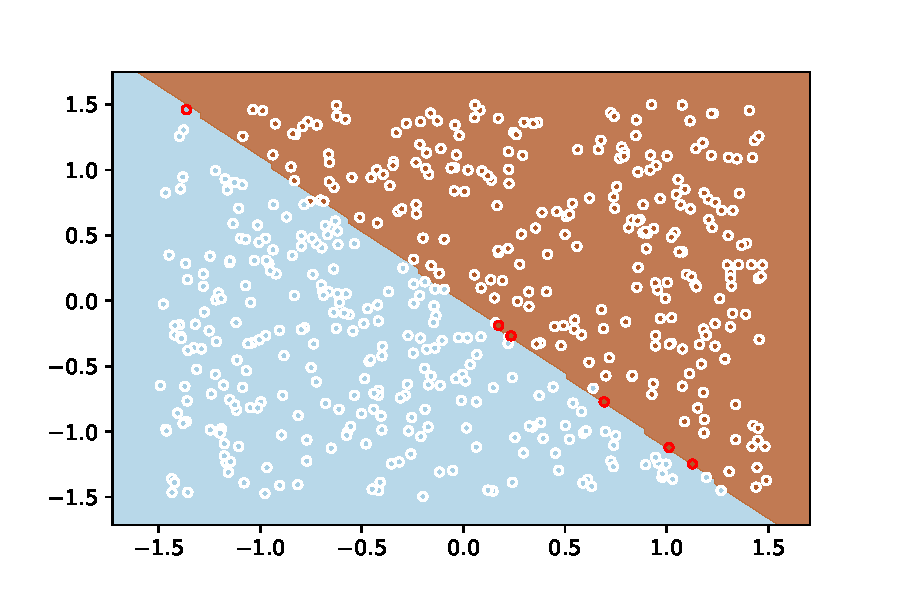
\includegraphics[scale=.6]{linearcase.pdf}
\end{center}
\end{itemize}
\end{frame}

\begin{frame}{Comparison to KNN, LDA, QDA}
Average Accuracy over one-hundred runs of linear case with 500 training samples and 500 testing samples:
\begin{itemize}
\item Linear SVM-Average: 0.98006012024
\item Linear LDA-Average: 0.97995991984
\item Linear QDA-Average: 0.979944583044
\item Linear KNN-Average: 0.979820465674
\end{itemize}
\end{frame}

\section{The Polynomial Case}
\subsection{Example Point Cloud}
\begin{frame}{Solving the Polynomial Case}
Objectives
\begin{itemize}
\item What's about the case where we can't just draw a straight line?
\item How do we draw a line through this set of samples?
\begin{center}
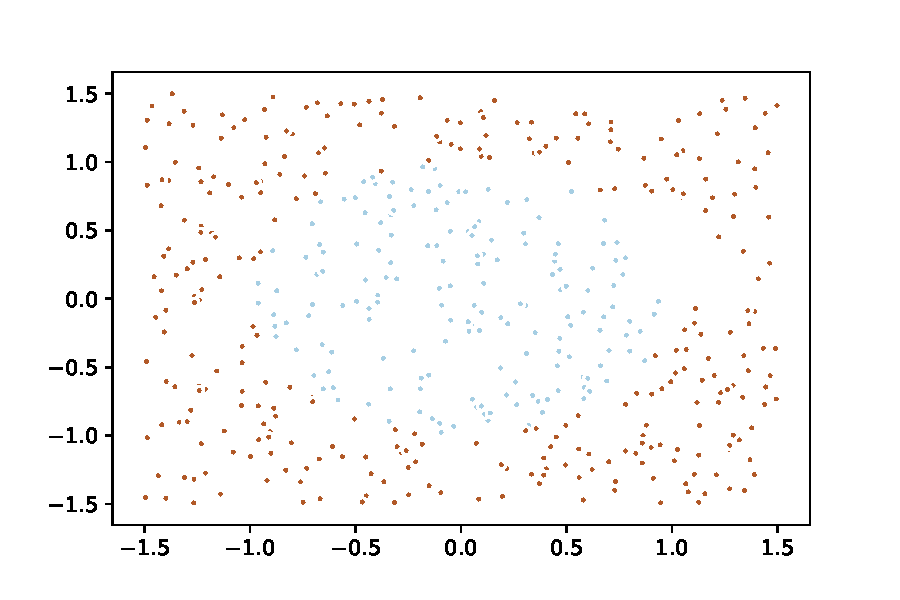
\includegraphics[scale=.6]{poly.pdf}
\end{center}
\end{itemize}
\end{frame}

\subsection{Introducing the Kernel Trick}
\begin{frame}{Kernel Trick}
Instead of maximizing $$v(\alpha) = \sum_i^n \alpha_i - \sum_i^n\sum_j^n \alpha_i \alpha_j y_i y_j \vec{x}_i^T \vec{x}_j$$
we maximize 
$$v(\alpha) = \sum_i^n \alpha_i - \sum_i^n\sum_j^n \alpha_i \alpha_j y_i y_j K(\vec{x}_i, \vec{x}_j)$$
where $K(\vec{x}_i, \vec{x}_j)$ is a function that maps two samples to some distance.
\end{frame}

\begin{frame}{Mercer's Condition and Example Kernels}
Mercer's Condition states that $K(\vec{x}_i, \vec{x}_j)$ must provide some measure of distance. This provides us with the means to develop a number of kernels.
\begin{itemize}
\item Linear Kernel: $\vec{x}_i^T\vec{x}_j + b$ where $b$ is some bias.
\item Polynomial Kernel: $(\vec{x}_i^T\vec{x}_j + b)^d$ where $b$ is some bias and $d$ is chosen dimension of polynomial
\item Radial Basis Kernel: $\exp\left[ \dfrac{||\vec{x}_i - \vec{x}_j ||^2}{2\sigma^2}   \right]$ where $\sigma$ is some smoothing factor.
\item Sigmoid Kernel: $\tanh(\gamma * \vec{x}_i^T\vec{x}_j + b)$ where $\gamma$ is chosen to maximize accuracy under a logistic model.
\end{itemize}
\end{frame}

\subsection{Results}
\begin{frame}{Results}
Choosing the polynomial kernel with dimension 2, we obtain the below results:
\begin{center}
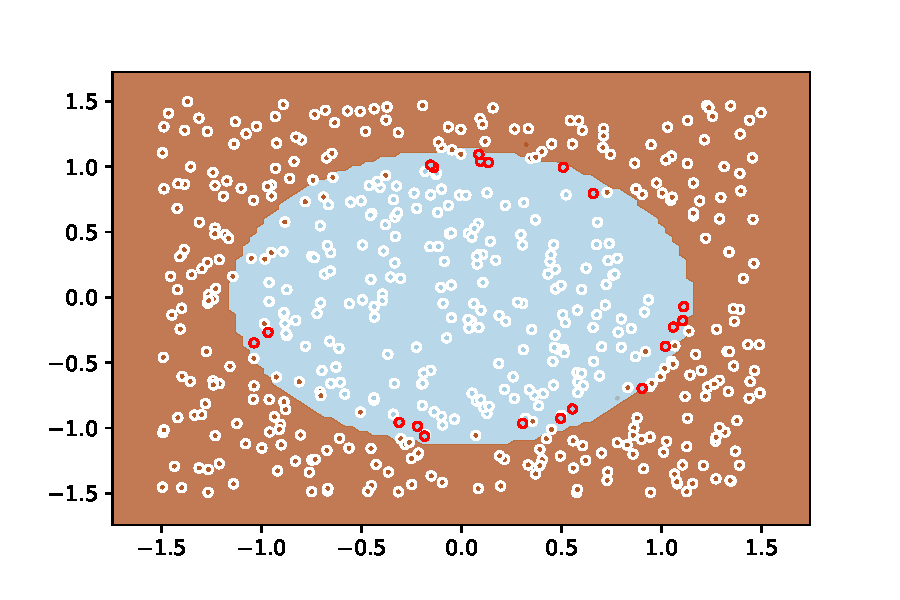
\includegraphics[scale=.6]{polynomialcase.pdf}
\end{center}
\end{frame}

\begin{frame}{Comparison to KNN, LDA, QDA}
Average Accuracy over one-hundred runs of linear case with 500 training samples and 500 testing samples:
\begin{itemize}
\item Polynomial SVM-Average: 0.837870741483
\item Polynomial LDA-Average: 0.83778668448
\item Polynomial QDA-Average: 0.837660013905
\item Polynomial KNN-Average: 0.837768320145
\end{itemize}
\end{frame}

\section{The Image Case (MNist Database)}

\begin{frame}{MNist Database -- Handwriting Digits}
Now that we've seen this on point clouds, we consider a set of images, specifically in this case handwriting.
\begin{itemize}
\item Utilizing the MNist Dataset\nocite{mnist} of hand-writing samples, I compare numbers labeled 5 and 1 to each other in an attempt to classify them from each other.
\item Example of this database's images below\nocite{lecun_bottou_bengio_haffner_1998}:
\begin{center}
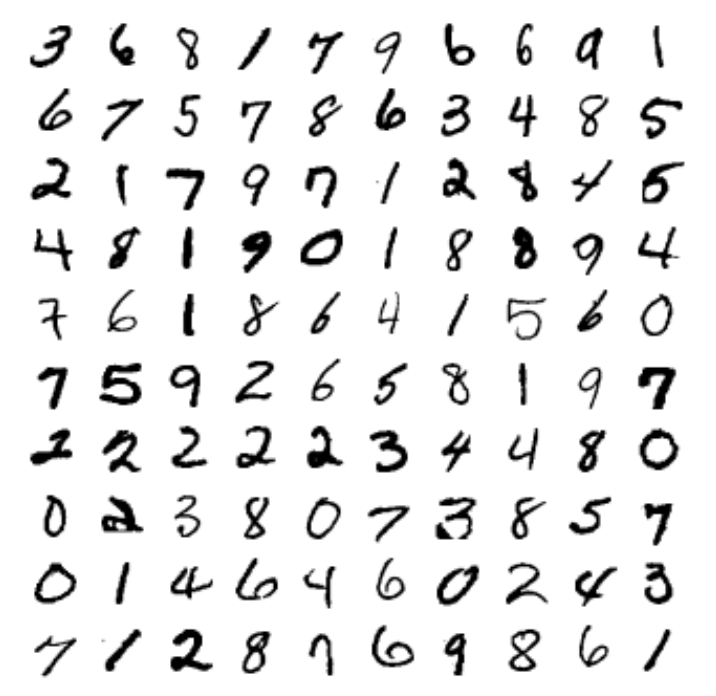
\includegraphics[scale=.3]{lecun}
\end{center}
\end{itemize}
\end{frame}

\begin{frame}{Results}
Using a polynomial-2 kernel, the following results were observed:
\begin{itemize}
\item With a training set of 12163 images of 1s or 5s and a testing set of 2027 images of 1s or 5s
\item Accuracy is approximately 100\%.
\item Computational time on a single core running at 2.6GHz was roughly 2 hours.
\item Would show images, but most are in ascii format and don't show well.
\item The algorithm can conclusively differentiate between the number 5 and the number 1.
\end{itemize}
\end{frame}


\section{Conclusion}

\begin{frame}{Strengths/Weaknesses of Support Vector Machines}
Strengths
\begin{itemize}
\item Popularized the "kernel trick" as a method for improving already used classification systems
\item Computationally efficient with $O(nd^2)$ where $n$ is number of samples and $d$ is number of dimensions.
\item Minimizing number of points needed for algorithm following quadratic maximization results in extremely fast prediction time
\item Able to form complex boundaries by use kernel trick
\end{itemize}
Weaknesses
\begin{itemize}
\item Primary weakness lies in weakness of kernel trick. For tasks such as facial recognition, multiple kernels are required which reduce accuracy compared to neural nets or clustering techniques.
\item Sets with large dimensions reduce the computational efficiency which lends to using our machine learning methods
\item Easily falls into over-fitting problems for difficult point clouds
\end{itemize}
\end{frame}


\begin{frame}{Future Work}
Items for future development
\begin{itemize}
\item One vs. All method for multiple classification (i.e. classifying on numbers 0-9 as opposed to 1 and 5)
\item Increased number of kernels for different tasks (such as facial classification or map identification)
\item Parallel Computing versions in order to handle larger datasets
\end{itemize}
\end{frame}



\begin{frame}{References}
\bibliography{citations.bib}
\bibliographystyle{plain}
\end{frame}




\end{document}